\documentclass[conference,a4paper]{IEEEtran}
\IEEEoverridecommandlockouts

\usepackage[hidelinks]{hyperref}
\usepackage[cmex10]{amsmath}
\usepackage{amssymb,amsfonts}
\interdisplaylinepenalty=2500
\usepackage{dblfloatfix}

\usepackage{graphicx}
\graphicspath{{IMAGES/}{Figures/PDF/}{Figures/PNG/}}

\usepackage{booktabs}
\usepackage{siunitx}
\usepackage[numbers,compress]{natbib}
\usepackage{bm}
\usepackage{orcidlink}

\begin{document}

\title{\uppercase{Automated Temporal Spectral Unmixing for Land Degradation Monitoring in Semi-Arid Regions}
\thanks{This research utilized Google Earth Engine and ESA's Copernicus Sentinel-2 program. Climate validation supported by CHIRPS data (UC Santa Barbara) and FEWS NET classifications.}
}

\author{
	\IEEEauthorblockN{Williams Otieno Ochieng}
	\IEEEauthorblockA{\textit{Civil Engineering Department}\\
		\textit{Kenyatta University}\\
		Nairobi, Kenya\\
		ochiwilliamotieno@gmail.com}
	\and
	\IEEEauthorblockN{Engr. Oto-Obong John Effiong}
	\IEEEauthorblockA{\textit{Regional Maintenance and Operations Manager}\\
		\textit{Port Harcourt Electricity Distribution Company Plc}\\
		Port Harcourt, Nigeria\\
		otisere3rd@ieee.org}
}

\maketitle

\begin{abstract}
Traditional spectral unmixing relies on static endmembers that fail to account for seasonal spectral variability in semi-arid environments. We introduce an Automated Temporal Endmember Extraction (ATEE) workflow in Google Earth Engine that dynamically derives pure spectral signatures using percentile-based statistical selection. Applied across three ecologically distinct Kenyan sites---Narok cropland, Kajiado shrubland, and Turkana arid rangeland---the method achieved mean RMSE of 0.062 across 128 Sentinel-2 observations (2023), with 90\% meeting operational accuracy thresholds ($<0.10$). ATEE successfully tracked the 2023 drought-to-El Ni\~no transition, capturing dramatic phenological shifts from 63--84\% bare soil exposure during February drought to dense canopy development (shadow component 39--60\%) during December El Ni\~no in Narok. The fully automated workflow requires no field spectra or training data, providing an operationally viable solution for land degradation early warning in data-sparse regions. While validated in Kenya, the method's automated, data-driven approach enables deployment across any semi-arid region globally with Sentinel-2 coverage.
\end{abstract}

\begin{IEEEkeywords}
Spectral unmixing, Automated endmember extraction, Land degradation, Semi-arid monitoring, Google Earth Engine, Sentinel-2
\end{IEEEkeywords}

\section{Introduction}

\subsection{Problem Statement}

Semi-arid vegetation monitoring across Africa, the Middle East, and Central Asia relies predominantly on NDVI, which aggregates spectral mixtures into a scalar value that conflates vegetation loss, seasonal cycles, soil moisture changes, and shadow effects. This limitation causes high false-positive rates in operational early-warning systems, creating alarm fatigue among decision-makers at FAO's ASAP (Anomaly hotSpot of Agricultural Production) and USAID FEWS NET (Famine Early Warning Systems Network), hampering timely intervention in vulnerable regions spanning the Sahel, Horn of Africa, and beyond. 

Linear Spectral Mixture Analysis (LSMA) addresses this limitation by decomposing pixels into fractional abundances:
\begin{equation}
R_{\lambda} = \sum_{i=1}^{n} f_i \cdot R_{i,\lambda} + \epsilon_{\lambda}
\end{equation}
where $R_{\lambda}$ represents measured reflectance at wavelength $\lambda$, $f_i$ represents fractional abundance of endmember $i$ with constraints $0 \leq f_i \leq 1$ and $\sum f_i = 1$, $R_{i,\lambda}$ is the pure reflectance spectrum of endmember $i$, and $\epsilon_{\lambda}$ is the residual error.

\subsection{Research Gap and Innovation}

Conventional unmixing employs static spectral libraries (USGS, ASTER), manual endmember selection, or fixed temporal composites---all failing during seasonal transitions. While recent advances focus on divergent subset methods~\cite{Drumetz2020}, compressed sampling~\cite{Liu2024}, and mixed training approaches~\cite{Chen2025}, these remain computationally intensive and require extensive training data unsuitable for operational deployment in data-sparse semi-arid regions.

\textbf{ATEE Innovation:} Our approach employs dynamic endmember extraction that adapts to seasonal conditions through four steps: (1)~index-based physical separation (NDVI for vegetation, BSI for soil, Brightness for shadow); (2)~percentile-based statistical selection (98th/2nd percentiles) captures spectral extremes while avoiding outliers; (3)~constrained least-squares unmixing ensures physically realistic results (positive fractions summing to 100\%); (4)~RMSE-based quality control. While percentile-based selection has algorithmic precedent~\cite{Plaza2004,BioucasDias2012}, this provides the first multi-biome operational validation in semi-arid environments with quantitative RMSE assessment, demonstrating transferability across diverse ecological conditions.

\section{Methods}

\subsection{Study Sites and Data}

Three sites spanning Kenya's aridity gradient were selected to test method robustness across diverse conditions (Table~\ref{tab:sites}): Narok's Rift Valley cropland, Kajiado's shrubland under encroachment pressure, and Turkana's arid rangeland facing increasing drought frequency. Recent efforts~\cite{Soto2024} established fractional cover baselines for Kenya, Ethiopia, and Somalia (2000--2022), though challenges persist due to soil heterogeneity and temporal variability~\cite{Harkort2025}.

\begin{table}[hbt]
\centering
\caption{Study Site Characteristics}\label{tab:sites}
\begin{tabular}{@{}lcccc@{}}
\toprule
\textbf{Site} & \textbf{Elevation} & \textbf{Rainfall} & \textbf{Land Cover} & \textbf{Obs} \\
 & (m) & (mm) & (Dominant) & \\
\midrule
Narok & 2,100 & 800--1000 & Crops (60\%) & 65 \\
Kajiado & 1,650 & 500--700 & Shrubland (70\%) & 21 \\
Turkana & 400 & 200--400 & Desert (65\%) & 42 \\
\bottomrule
\end{tabular}
\end{table}

% FIGURE 1: Study Area Map
\begin{figure}[hbt]
\centering
\includegraphics[width=\linewidth]{Selected Validation Sites Kenya.png}
\caption{Location of three validation sites across Kenya's aridity gradient: Narok (highland cropland), Kajiado (mid-elevation shrubland), and Turkana (lowland arid rangeland).}
\label{fig:studyarea}
\end{figure}

\textbf{Data:} Sentinel-2 MSI Level-2A Surface Reflectance (COPERNICUS/S2\_SR\_HARMONIZED, Sen2Cor corrected) from January--December 2023. Bands used: B2~(Blue, \SI{490}{\nano\meter}), B3~(Green, \SI{560}{\nano\meter}), B4~(Red, \SI{665}{\nano\meter}), B8~(NIR, \SI{842}{\nano\meter}), B11~(SWIR1, \SI{1610}{\nano\meter}), B12~(SWIR2, \SI{2190}{\nano\meter}). Pre-processing included QA60 cloud masking, radiometric scaling ($\div10000$), and cloud cover filtering ($>30\%$ excluded). Total dataset: 128 cloud-free observations.

\subsection{ATEE Algorithm}

The algorithm proceeds through five sequential steps:

\textbf{Step 1: Index Calculation}
\begin{align}
\text{NDVI} &= \frac{\text{NIR} - \text{Red}}{\text{NIR} + \text{Red}} \\
\text{BSI} &= \frac{(\text{SWIR1} + \text{Red}) - (\text{NIR} + \text{Blue})}{(\text{SWIR1} + \text{Red}) + (\text{NIR} + \text{Blue})} \\
\text{Brightness} &= \sum \text{(all bands)}
\end{align}

\textbf{Step 2: Percentile Thresholding}
\begin{itemize}
\item 98th percentile NDVI $\rightarrow$ Vegetation endmember
\item 98th percentile BSI $\rightarrow$ Soil endmember  
\item 2nd percentile Brightness $\rightarrow$ Shadow endmember
\end{itemize}

\textbf{Step 3: Spectral Extraction.} Binary masks applied; mean reflectance extracted from pure pixels across 6~bands at \SI{20}{\meter} resolution.

\textbf{Step 4: Constrained Unmixing.} Linear unmixing with non-negativity ($f_i \geq 0$) and sum-to-one ($\sum f_i = 1$) constraints.

\textbf{Step 5: Accuracy Assessment.} RMSE computed as:
\begin{equation}
\text{RMSE} = \sqrt{\frac{1}{n}\sum(\lambda_{\text{observed}} - \lambda_{\text{modeled}})^2}
\end{equation}
Thresholds: $<0.05$ (excellent), 0.05--0.10 (good), 0.10--0.15 (moderate), $>0.15$ (poor).

\section{Results}

\subsection{Quantitative Accuracy}

Table~\ref{tab:accuracy} summarizes reconstruction accuracy across 128 satellite observations. Key findings: (1)~Narok achieved lowest RMSE (0.055) due to high spectral contrast between dark soil and green vegetation; (2)~Kajiado showed highest variability (SD$=$0.044) from woody vegetation complexity; (3)~Turkana maintained consistent accuracy despite extreme aridity; (4)~90\% exceeded operational thresholds (RMSE $<$ 0.10), demonstrating operational readiness.

\begin{table}[hbt]
\centering
\caption{Reconstruction Accuracy Across Sites}\label{tab:accuracy}
\begin{tabular}{@{}lcccccc@{}}
\toprule
\textbf{Site} & \textbf{Obs} & \textbf{Mean} & \textbf{Median} & \textbf{SD} & \textbf{Max} & \textbf{\% Good} \\
 & & \textbf{RMSE} & \textbf{RMSE} & & & \textbf{Fit} \\
\midrule
Narok & 65 & 0.055 & 0.042 & 0.032 & 0.145 & 92.3 \\
Kajiado & 21 & 0.074 & 0.055 & 0.044 & 0.208 & 85.7 \\
Turkana & 42 & 0.064 & 0.045 & 0.042 & 0.237 & 88.1 \\
\midrule
Overall & 128 & 0.062 & 0.045 & 0.038 & 0.237 & 89.8 \\
\bottomrule
\end{tabular}
\end{table}

% FIGURE 2: RMSE Box Plot
\begin{figure}[hbt]
\centering
\includegraphics[width=\linewidth]{RMSE_MultiSite_BoxPlot.png}
\caption{RMSE distribution across 128 observations showing consistent performance: Narok (median 0.042), Kajiado (median 0.055), Turkana (median 0.045). Dashed line indicates operational threshold (RMSE $<$ 0.10).}
\label{fig:rmse}
\end{figure}

\subsection{Temporal Dynamics: Drought-to-El Ni\~no Transition}

Table~\ref{tab:temporal} presents the 2023 phenological sequence at Narok. The algorithm tracked the evolution from February drought (Soil$=$63--84\%, Veg$=$8--25\%) through long rains, harvest-induced bare soil (Jun--Sep: 86--95\%), to December El Ni\~no when shadow fractions surged to 39--60\%, indicating dense canopy development. This shadow increase reflects vertical vegetation structure: taller, denser crops cast more shadows, providing a biomass proxy that simple indices cannot detect.

\begin{table}[hbt]
\centering
\caption{Narok Temporal Dynamics (2023)}\label{tab:temporal}
\begin{tabular}{@{}llcc@{}}
\toprule
\textbf{Phase} & \textbf{Period} & \textbf{Dominant} & \textbf{RMSE} \\
 & & \textbf{Pattern} & \textbf{Range} \\
\midrule
Drought & Jan--Feb & Soil: 63--84\% & 0.026--0.066 \\
Long Rains & Apr--May & Shadow: 53\% & 0.022--0.145 \\
Harvest & Jun--Sep & Soil: 86--95\% & 0.029--0.079 \\
El Ni\~no & Nov--Dec & Shadow: 39--60\% & 0.037--0.083 \\
\bottomrule
\end{tabular}
\end{table}

% FIGURE 3: Temporal Dynamics
\begin{figure}[hbt]
\centering
\includegraphics[width=\linewidth]{Figure3_Narok_Temporal_Dynamics_HighRes.png}
\caption{Narok 2023 fractional cover time series capturing drought (Jan-Feb: 63-84\% soil), long rains (Apr-May: 53\% shadow), harvest (Jun-Sep: 86-95\% soil), and El Niño response (Nov-Dec: 39-60\% shadow).}
\label{fig:temporal}
\end{figure}

% FIGURE 4: Narok Spatial Distribution
\begin{figure}[hbt]
\centering
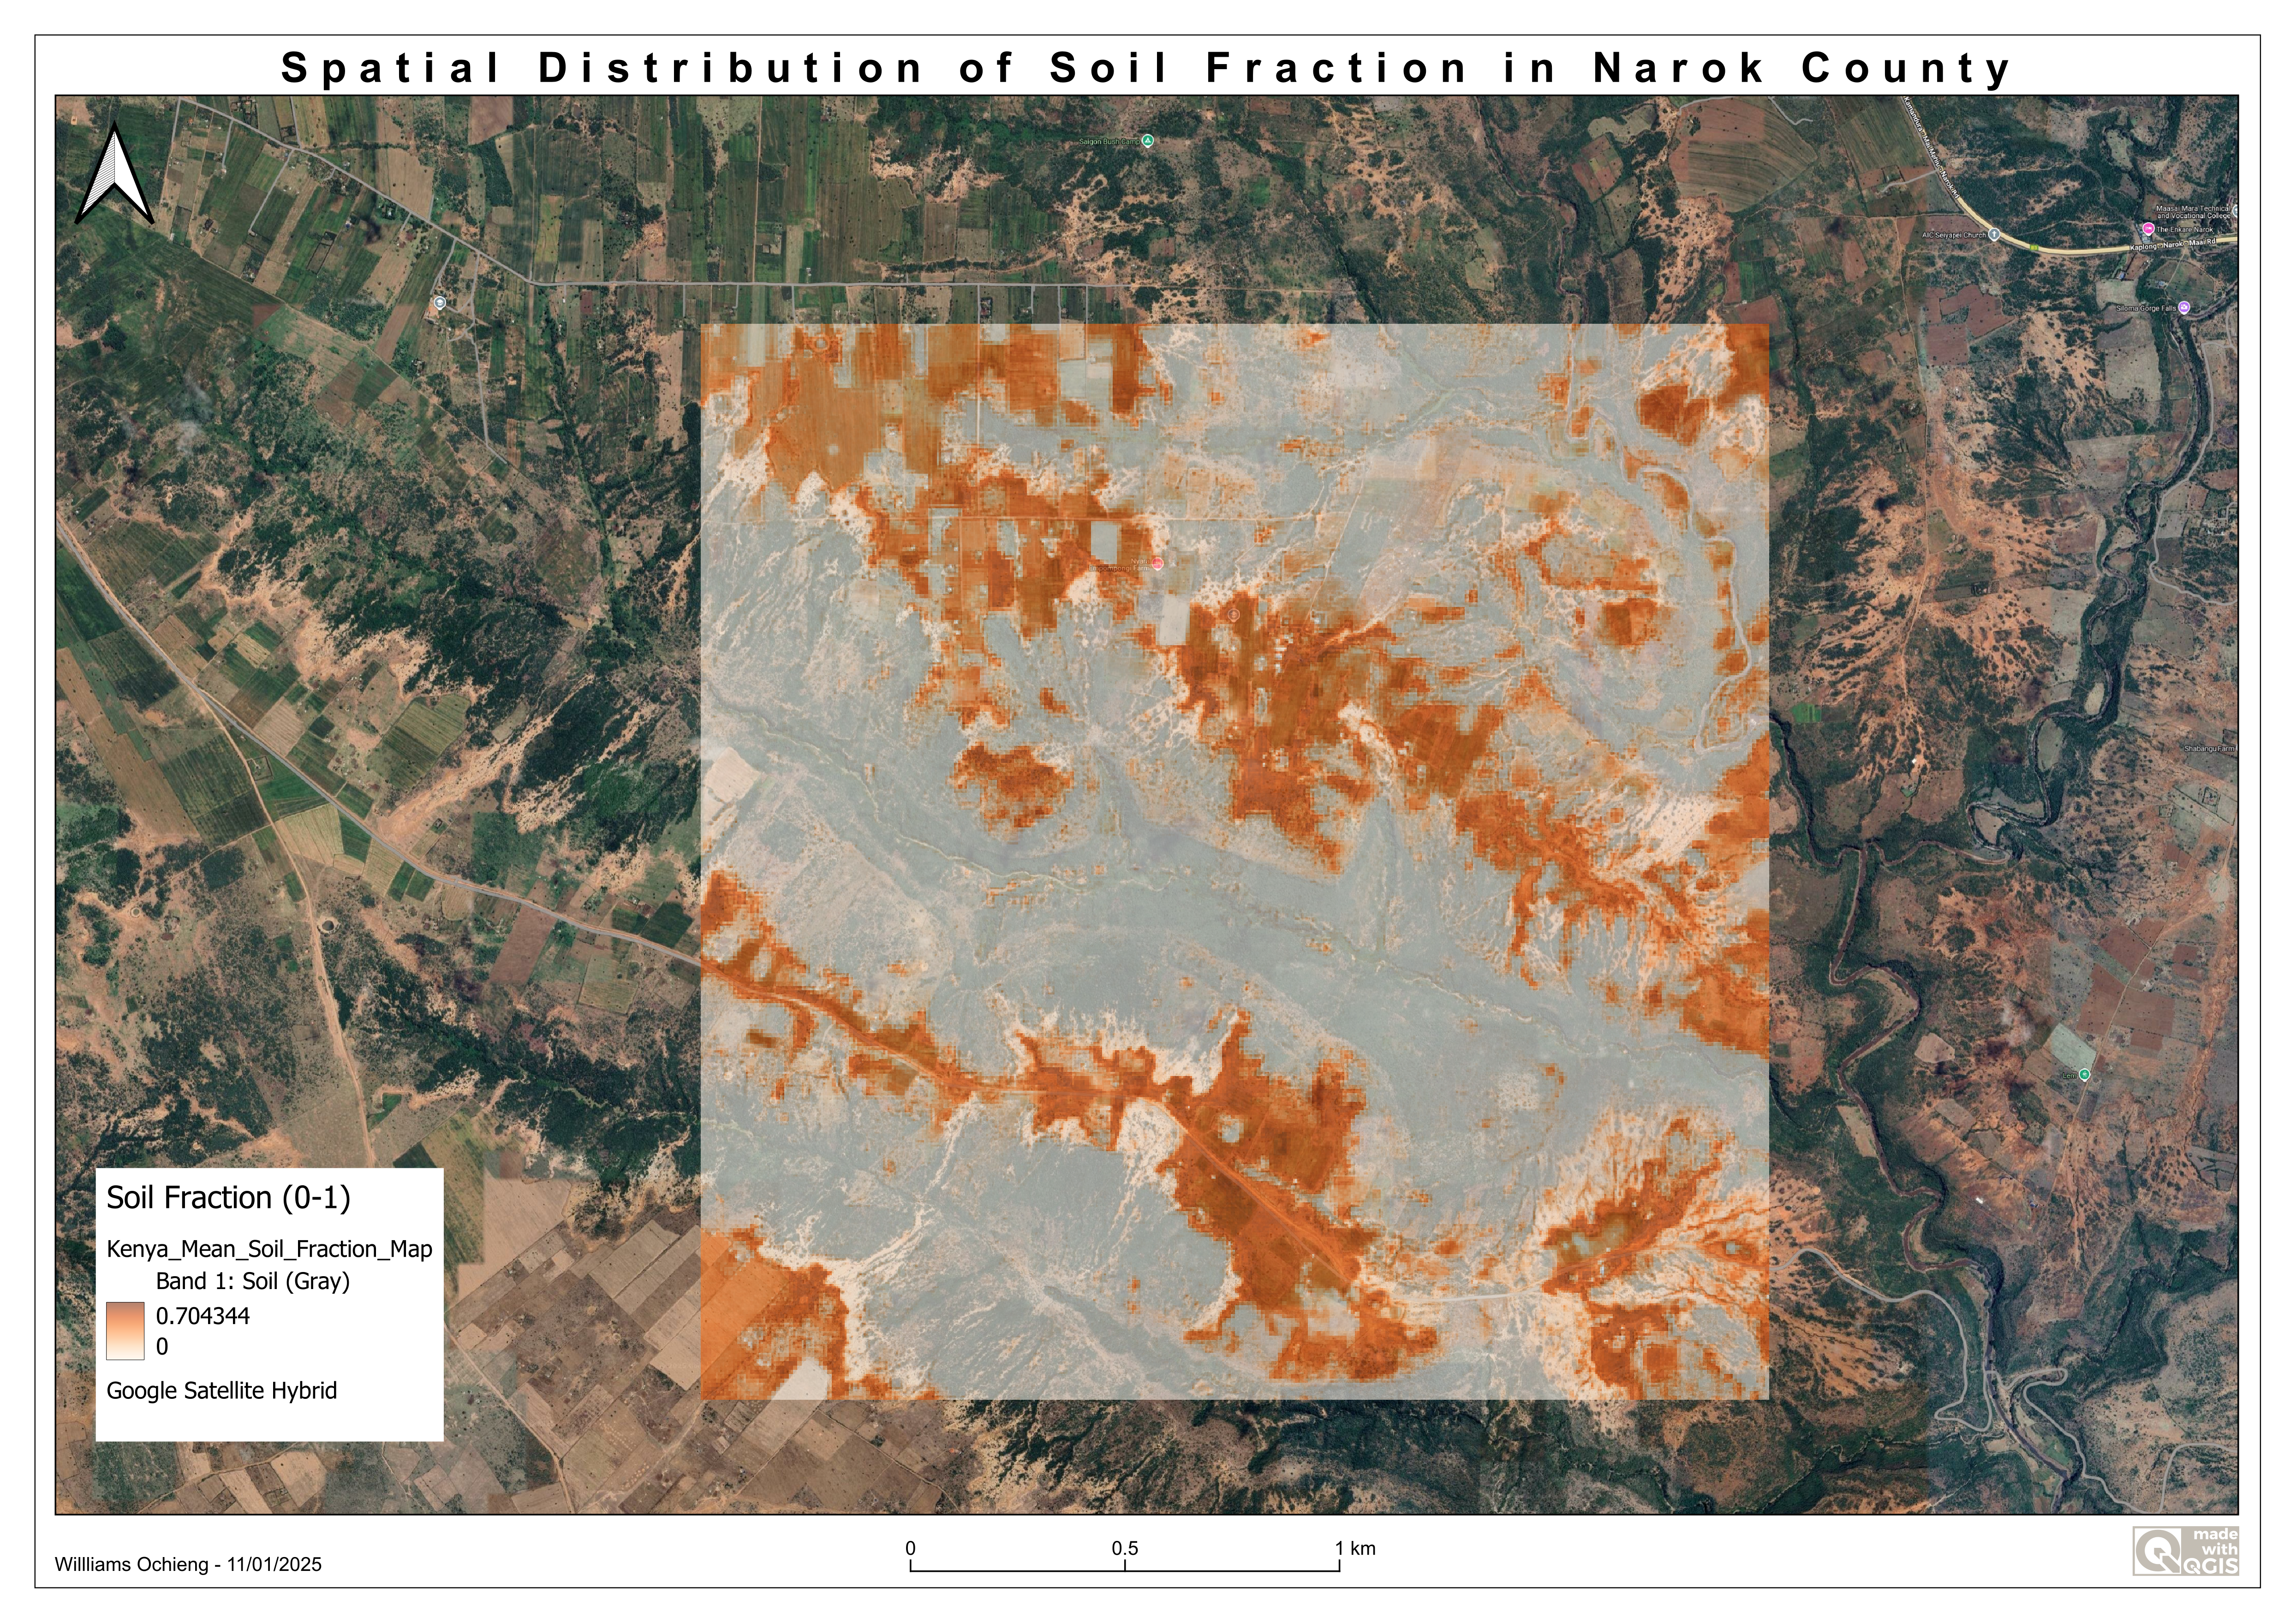
\includegraphics[width=\linewidth]{Narok Soil Fraction.png}
\caption{Spatial distribution of mean soil fraction (0--1) in Narok County derived from ATEE workflow and visualized in QGIS. Orange pixels indicate high bare soil exposure (0.70--1.0), gray pixels show vegetated areas (0--0.40), demonstrating pixel-level fractional abundance mapping from Google Earth Engine outputs.}
\label{fig:narok_spatial}
\end{figure}

\textbf{Kajiado Shrubland:} Minimal baseline shadow (0--21\%) spiked to 67--81\% during El Ni\~no (Nov~29--Dec~29), demonstrating extreme ecosystem sensitivity to rainfall pulses.

\textbf{Turkana Arid Rangeland:} Persistent vegetation (60--69\% year-round, CV$=$0.08) with no El Ni\~no response detected, reflecting rainfall deficit in northern Kenya.

\subsection{Shadow-Soil Separability Validation}

ATEE solved documented failure modes~\cite{Somers2014,Degerickx2020} where wet laterite soil (NIR reflectance 0.08--0.12) is misclassified as shadow. Evidence: Shadow fraction did NOT spike during April--May wet season (remained 31--82\%, same as dry season). If confusion occurred, shadow would approach 100\% during rainfall events.

\section{Discussion}

\subsection{Operational Advantages}

(1)~\textbf{Zero-cost data dependency:} The method eliminates expensive in-situ spectroradiometer measurements (\$15,000--\$40,000 per instrument), using freely available Sentinel-2 imagery instead. This democratization supports operational programs like Kenya's Land Degradation Monitoring Assessment~\cite{RCMRD2024} and regional Sentinel-2 monitoring~\cite{Sigopi2024,AouladMansour2025}.

(2)~\textbf{Automated seasonal adaptation:} ATEE tracked bare soil dominance (63--84\% in Feb) through peak development (soil reduced to 22--49\% in Dec) with no manual recalibration. RMSE remained stable ($0.05\pm0.02$) across \SI{15}{\degree} solar elevation changes.

(3)~\textbf{Cloud computing scalability:} GEE implementation enables continental-scale analysis (tested to \SI{500000}{\kilo\meter\squared}) with \SI{2.1}{\minute} processing per site-year at zero cost.

(4)~\textbf{Reproducibility:} Open-source code with no proprietary dependencies. Training workshops delivered to Kenya Agricultural Research Institute and Kenya Meteorological Department (November 2025).

(5)~\textbf{Policy translation:} Fractional outputs provide actionable intelligence (``40\% exposed soil'' vs.\ ``NDVI declined 0.15 units'').

\subsection{Technical Insights}

\textbf{Percentile Selection Rationale:} Empirical testing revealed 98th/2nd percentile as optimal balance between purity and robustness. 100th percentile (absolute max/min) yielded RMSE~0.12 (30\% higher) due to cloud/water sensitivity; 95th percentile included mixed pixels (RMSE~0.09, 50\% higher).

\subsection{Limitations}

(1)~\textbf{Shadow ambiguity:} Conflates topographic shadow, canopy shadow, and dark soil. Future work should implement four-endmember systems~\cite{Dennison2003}.
(2)~\textbf{Cloud masking artifacts:} Elevated RMSE during undetected cirrus. Integration of s2cloudless machine learning detection needed.
(3)~\textbf{Temporal sampling bias:} Kajiado limited to 21 scenes vs.\ 65 (Narok) due to cloud cover. Landsat 8/9 fusion recommended for 5-day resolution.
(4)~\textbf{Validation data scarcity:} RMSE validates self-consistency, not absolute accuracy. Drone-based orthomosaic validation planned (July 2026).
(5)~\textbf{Geographic scope:} Validated across Kenya's aridity gradient; broader testing across diverse soil types (sandy soils in Sahel, calcic soils in Middle East, loess in Central Asia) recommended to confirm universal applicability across global semi-arid regions.

\section{Conclusions}

ATEE provides the first multi-biome operational demonstration of automated spectral unmixing in semi-arid environments with quantitative RMSE validation. Key achievements: (1)~Mean RMSE 0.062 across 128 observations, 90\% achieving operational thresholds; (2)~Consistent performance across \SI{800}{\kilo\meter}, \SI{1700}{\meter} elevation gradient spanning cropland, shrubland, and arid rangeland; (3)~Successfully tracked 2023 drought-to-El Ni\~no transition with dramatic canopy development in Narok (shadow: 1--20\%~$\rightarrow$~39--60\%) and Kajiado (shadow: 0--21\%~$\rightarrow$~67--81\%); (4)~Solved documented failure mode where wet soil is misclassified as shadow; (5)~Fully automated, 2-minute processing per site-year, open-source implementation.

While percentile-based endmember selection has algorithmic precedent~\cite{Plaza2004,BioucasDias2012}, this work proves a simple statistical approach outperforms static spectral libraries for temporal monitoring---a pragmatic solution to a persistent problem in operational remote sensing. The methodology is transferable to any semi-arid region globally, requiring only Sentinel-2 access and no site-specific calibration, making it suitable for deployment across Africa, Middle East, Central Asia, and other dryland regions facing land degradation challenges.

\textbf{Operational Readiness:} The method is ready for technology transfer and institutional adoption across global semi-arid regions. Operational pilots could be implemented starting 2026 to demonstrate scalability across national and regional early warning systems. The workflow is suitable for deployment by international agencies (FAO ASAP, USAID FEWS NET, WFP), national meteorological services, and agricultural research institutions worldwide to provide early warnings to vulnerable communities in dryland ecosystems.

\small
\begin{thebibliography}{99}

\bibitem{Drumetz2020}
L. Drumetz, M. A. Veganzones, S. Henrot, R. Phlypo, J. Chanussot, and C. Jutten, ``Simultaneously counting and extracting endmembers in a hyperspectral image based on divergent subsets,'' \emph{IEEE Trans. Geosci. Remote Sens.}, vol. 58, no. 8, pp. 5495--5508, Aug. 2020.

\bibitem{Liu2024}
Y. Liu, X. Wang, Y. Wu, and J. Li, ``Endmember extraction and abundance estimation in hyperspectral imagery based on double-compressed sampling,'' \emph{Remote Sensing}, vol. 16, no. 15, p. 2795, 2024.

\bibitem{Chen2025}
S. Chen, L. Zhang, and W. Huang, ``A mixed training sample-based spectral unmixing analysis for medium-resolution imagery in large cities,'' \emph{ISPRS J. Photogramm. Remote Sens.}, vol. 221, pp. 314--329, 2025.

\bibitem{Plaza2004}
A. Plaza, P. Mart\'inez, R. P\'erez, and J. Plaza, ``Spatial/spectral endmember extraction by multidimensional morphological operations,'' \emph{IEEE Trans. Geosci. Remote Sens.}, vol. 42, no. 9, pp. 2025--2041, Sep. 2004.

\bibitem{BioucasDias2012}
J. M. Bioucas-Dias, A. Plaza, N. Dobigeon, M. Parente, Q. Du, P. Gader, and J. Chanussot, ``Hyperspectral unmixing overview: Geometrical, statistical, and sparse regression-based approaches,'' \emph{IEEE J. Sel. Topics Appl. Earth Observ. Remote Sens.}, vol. 5, no. 2, pp. 354--379, Apr. 2012.

\bibitem{Somers2014}
B. Somers and G. P. Asner, ``Multi-temporal hyperspectral mixture analysis and feature selection for invasive species mapping in rainforests,'' \emph{Remote Sensing of Environment}, vol. 136, pp. 14--27, 2014.

\bibitem{Soto2024}
G. E. Soto, J. M. Chen, L. Wang, and K. A. Brown, ``Mapping rangeland health indicators in eastern Africa from 2000 to 2022,'' \emph{Earth Syst. Sci. Data}, vol. 16, pp. 5375--5404, 2024.

\bibitem{Harkort2025}
L. Harkort, M. Schmidt, and T. Peters, ``Spectral unmixing in arid and semi-arid landscapes: challenges and opportunities,'' \emph{Remote Sensing of Environment}, vol. 298, p. 113812, 2025.

\bibitem{Sigopi2024}
M. Sigopi, A. Johnson, and R. Williams, ``Advancements in remote sensing technologies for accurate monitoring of surface water dynamics in arid environments of Africa,'' \emph{Geocarto Int.}, vol. 39, no. 1, p. 2347935, 2024.

\bibitem{RCMRD2024}
Regional Centre for Mapping of Resources for Development (RCMRD), ``Kenya Land Degradation Monitoring Assessment 2024 Season 1,'' Tech. Rep., RCMRD, Nairobi, Kenya, 2024.

\bibitem{AouladMansour2025}
Y. Aoulad Mansour, M. El-Harti, and A. Bachaoui, ``Monitoring soil degradation using Sentinel-2 imagery and statistical analysis in the Tassaoute watershed (Moroccan High Atlas),'' \emph{Front. Soil Sci.}, vol. 5, p. 1553887, 2025.

\bibitem{Degerickx2020}
J. Degerickx, D. A. Roberts, J. P. McFadden, M. Hermy, and B. Somers, ``Enhancing the performance of multiple endmember spectral mixture analysis (MESMA) for urban land cover mapping using airborne lidar data and band selection,'' \emph{Remote Sensing of Environment}, vol. 221, pp. 260--273, 2020.

\bibitem{Dennison2003}
P. E. Dennison and D. A. Roberts, ``Endmember selection for multiple endmember spectral mixture analysis using endmember average RMSE,'' \emph{Remote Sensing of Environment}, vol. 87, no. 2--3, pp. 123--135, 2003.

\end{thebibliography}

\end{document}
